
%!TEX root = ../thesis.tex
%*******************************************************************************
%****************************** Second Chapter *********************************
%*******************************************************************************

\chapter{Background}

\ifpdf
    \graphicspath{{Chapter2/Figs/Raster/}{Chapter2/Figs/PDF/}{Chapter2/Figs/}}
\else
    \graphicspath{{Chapter2/Figs/Vector/}{Chapter2/Figs/}}
\fi



\vspace*{\fill} 
\begin{quote} 
\centering 
\textit{“When an axon of cell A is near enough to excite a cell B and repeatedly or persistently takes part in firing it, some growth process or metabolic change takes place in one or both cells such that A’s efficiency, as one of the cells firing B, is increased.” - Hebb’s Rule}
\end{quote}
\vspace*{\fill}

\section{Neural Networks}
\subsection{Brain Analogies}

A psychologist, Rosenblatt conceived of the Percetron as a simplified mathematical model of how the neurons in our brains operate: it takes a set of binary inputs (nearby neurons), multiplies each input by a continuous valued weight (the synapse strength to each nearby neuron), and thresholds the sum of these weighted inputs to output a 1 if the sum is big enough and otherwise a 0 (in the same way neurons either fire or do not).

\begin{figure}[H]
\begin{center}
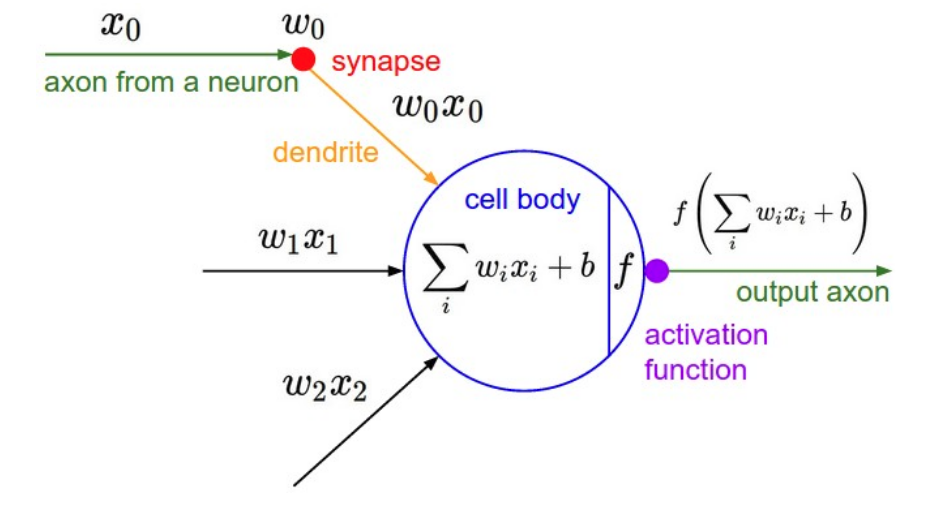
\includegraphics[height=.28\textheight]{Chapter2/Figs/NeuralNetwork.png}
\label{fig:Neural_Network}
\caption{Biologically inspired Neural Network \cite{karparthy}}
\end{center}
\end{figure}

\subsection{Artificial Neural Network}

An Artificial Neural Network (ANN) is an information processing paradigm that is inspired by the way biological nervous systems, such as the brain, process information. The key element of this paradigm is the novel structure of the information processing system. It is composed of a large number of highly interconnected processing elements (neurons) working in unison to solve specific problems. ANNs, like people, learn by example. An ANN is configured for a specific application, such as pattern recognition or data classification, through a learning process. Learning in biological systems involves adjustments to the synaptic connections that exist between the neurons. This is true of ANNs as well.


Neural networks consist of input and output layers, as well as (in most cases) a hidden layer consisting of units that transform the input into something that the output layer can use. They are excellent tools for finding patterns which are far too complex or numerous for a human programmer to extract and teach the machine to recognize.


\begin{figure}[H]
\begin{center}
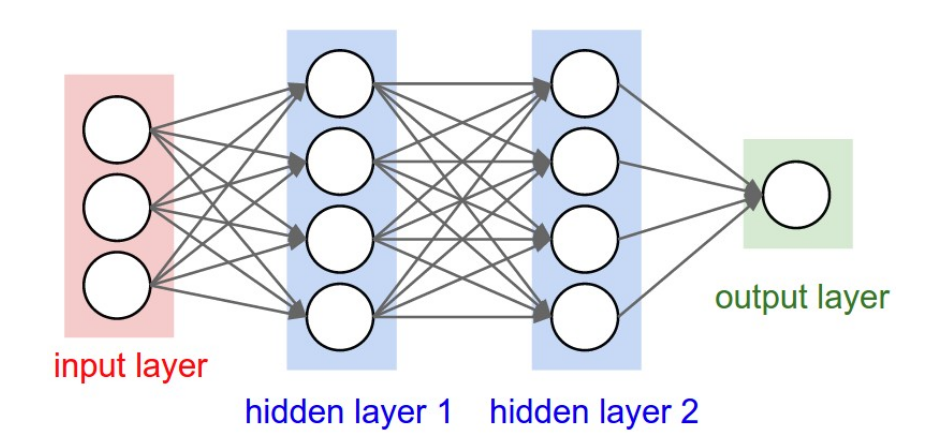
\includegraphics[height=.28\textheight]{Chapter2/Figs/TwoLayeredNN.png}
\label{fig:Two Layered Neural_Network}
\caption{Neural Network with two hidden layers \cite{karparthy}}
\end{center}
\end{figure}


\subsection{Convolutional Neural Network}

“According to the hierarchy model by Hubel and Wiesel, the neural network in the visual cortex has a hierarchy structure: LGB (lateral geniculate body)->simple cells->complex cells->lower order hypercomplex cells->higher order hypercomplex cells. It is also suggested that the neural network between lower order hypercomplex cells and higher order hypercomplex cells has a structure similar to the network between simple cells and complex cells. In this hierarchy, a cell in a higher stage generally has a tendency to respond selectively to a more complicated feature of the stimulus pattern, and, at the same time, has a larger receptive field, and is more insensitive to the shift in position of the stimulus pattern. … Hence, a structure similar to the hierarchy model is introduced in our model.”

Or, more concretely: the first hidden layer of the neural net was convolutional - instead of each neuron having a different weight for each pixel of the input image (40x60=2400 weights), the neurons only have a small set of weights (5x5=25) that were applied a whole bunch of small subsets of the image of the same size. So, for instance instead of having 4 different neurons learn to detect 45 degree lines in each of the 4 corners of the input image, a single neuron could learn to detect 45 degree lines on subsets of the image and do that everywhere within it. Layers past the first work in a similar way, but take in the ‘local’ features found in the previous hidden layer rather than pixel images, and so ‘see’ successively larger portions of the image since they are combining information about increasingly larger subsets of the image. Finally, the last two layers are just plain normal neural net layers that use the higher-order larger features generated by the convolutional layers to determine which digit the input image corresponds to.

The reason for why this is helpful is intuitively if not mathematically clear: without such constraints the network would have to learn the same simple things (such as detecting 45 degree lines, small circles, etc) a whole bunch of times for each portion of the image. But with the constraint there, only one neuron would need to learn each simple feature - and with far fewer weights overall, it could do so much faster! Moreover, since the pixel-exact locations of such features do not matter the neuron could basically skip neighboring subsets of the image - subsampling, now known as a type of pooling - when applying the weights, further reducing the training time. The addition of these two types of layers - convolutional and pooling layers - are the primary distinctions of Convolutional Neural Nets (CNNs/ConvNets) from plain old neural nets.


\section{Probabilistic Machine Learning}
\subsection{Variational Inference}

Performing Bayesian inference on a neural network requires the posterior distribution of the network weights given the data. If the weights have a prior probability P (w\textbar{}α) that depends on some parameters α, the posterior can be written Pr(w\textbar{}D, α). Unfortunately, for most neural networks Pr(w\textbar{}D, α) cannot be calculated analytically, or even efficiently sampled from. Variational inference addresses this problem by approximating Pr(w\textbar{}D, α) with a more tractable distribution Q (w\textbar{}β). The approximation is fitted by minimising the variational free energy F with respect to the parameters
β, where\\ 
F = − ln  Pr(D\textbar{}w)P (w\textbar{}α) Q (w\textbar{}β) 
w∼Q(β)\\
and for some function g of a random variable x with distribution p(x),
hgix∼p denotes the expectation\\
of g over p. A fully Bayesian approach would infer the prior parameters
α from a hyperprior; however in this paper they are found by simply
minimising F with respect to α as well as β.

\subsection{Monte  Carlo  variational  inference}
\subsection{Local  reparametrisation  trick}

We utilise the local reparameterization trick \cite{kingma2015variational} and apply it to \acp{cnn}. Following \cite{kingma2015variational,neklyudov2018variance}, we do not sample the weights $w$, but we sample instead layer activations $b$ due to its consequent computational acceleration. The variational posterior probability distribution $q_{\theta}(w_{ijhw}|\mathcal{D})=\mathcal{N}(\mu_{ijhw},\alpha_{ijhw}\mu^2_{ijhw})$ (where $i$ and $j$ are the input, respectively output layers, $h$ and $w$ the height, respectively width of any given filter) allows to implement the local reparamerization trick in convolutional layers. This results in the subsequent equation for convolutional layer activations $b$:
\begin{equation}
    b_j=A_i\ast \mu_i+\epsilon_j\odot \sqrt{A^2_i\ast (\alpha_i\odot \mu^2_i)}
\end{equation}
where $\epsilon_j \sim \mathcal{N}(0,1)$, $A_i$ is the receptive field, $\ast$ signalises the convolutional operation, and $\odot$ the component-wise multiplication.

\section{Bayes by Backprop}
\textit{Bayes by Backprop} \cite{graves2011practical, blundell2015weight} is a variational inference method to learn the posterior distribution on the weights $w \sim q_{\theta}(w|\mathcal{D})$ of a neural network from which weights $w$ can be sampled in backpropagation. 
It regularises the weights by minimising a compression cost, known as the variational free energy or the expected lower bound on the marginal likelihood.

Since the true posterior is typically intractable, an approximate distribution $q_{\theta}(w|\mathcal{D})$ is defined that is aimed to be as similar as possible to the true posterior $p(w|\mathcal{D})$, measured by the Kullback-Leibler (KL) divergence \cite{kullback1951information}. Hence, we define the optimal parameters $\theta^{opt}$ as
\begin{equation}
    \begin{aligned} \label{KL}
        \theta^{opt}&=\underset{\theta}{\text{arg min}}\ \text{KL} \ [q_{\theta}(w|\mathcal{D})\|p(w|\mathcal{D})] \\
        &=\underset{\theta}{\text{arg min}}\ \text{KL} \ [q_{\theta}(w|\mathcal{D})\|p(w)] \\ & -\mathbb{E}_{q(w|\theta)}[\log p(\mathcal{D}|w)]+\log p(\mathcal{D})
    \end{aligned}
\end{equation}

where
\begin{equation}
    \text{KL} \ [q_{\theta}(w|\mathcal{D})\|p(w)]= \int q_{\theta}(w|\mathcal{D})\log\frac{q_{\theta}(w|\mathcal{D})}{p(w)}dw .
\end{equation}
This derivation forms an optimisation problem with a resulting cost function widely known as \textit{variational free energy} \cite{neal1998view,yedidia2005constructing,friston2007variational} which is built upon two terms: the former, $\text{KL} \ [q_{\theta}(w|\mathcal{D})\|p(w)]$, is dependent on the definition of the prior $p(w)$, thus called complexity cost, whereas the latter, $\mathbb{E}_{q(w|\theta)}[\log p(\mathcal{D}|w)]$, is dependent on the data $p(\mathcal{D}|w)$, thus called likelihood cost. 
The term $\log p(\mathcal{D})$ can be omitted in the optimisation because it is constant.
\newline Since the KL-divergence is also intractable to compute exactly, we follow a stochastic variational method \cite{graves2011practical,blundell2015weight}.
We sample the weights $w$ from the variational distribution $q_{\theta}(w|\mathcal{D})$ since it is much more probable to draw samples which are appropriate for numerical methods from the variational posterior $q_{\theta}(w|\mathcal{D})$ than from the true posterior $p(w|\mathcal{D})$. Consequently, we arrive at the tractable cost function \eqref{cost} which is aimed to be optimized, i.e. minimised w.r.t. $\theta$, during training:
\begin{equation} \label{cost}
    \mathcal{F}(\mathcal{D}, \theta)\approx \sum_{i=1}^n \log q_{\theta}(w^{(i)}|\mathcal{D})-\log p(w^{(i)})-\log p(\mathcal{D}|w^{(i)})
\end{equation}
%
where $n$ is the number of draws.
\newline We sample $w^{(i)}$ from $q_{\theta}(w|\mathcal{D})$. The uncertainty afforded by \textit{Bayes by Backprop} trained neural networks has been used successfully for training feedforward neural networks in both supervised and reinforcement learning environments \cite{blundell2015weight,lipton2016efficient,houthooft2016curiosity}, for training recurrent neural networks \cite{fortunato2017bayesian}, but has not been applied to convolutional neural networks to-date.

